% ---------------------------------------------------------------------
% The NeurIPS 2026 style file is embedded below so this single file
% compiles anywhere (Overleaf included) with no separate upload.
% ---------------------------------------------------------------------
\begin{filecontents*}[overwrite]{neurips_2026.sty}
% partial rewrite of the LaTeX2e package for submissions to the
% Conference on Neural Information Processing Systems (NeurIPS):
%
% - uses more LaTeX conventions
% - line numbers at submission time replaced with aligned numbers from
%   lineno package
% - \nipsfinalcopy replaced with [final] package option
% - automatically loads times package for authors
% - loads natbib automatically; this can be suppressed with the
%   [nonatbib] package option
% - adds foot line to first page identifying the conference
% - adds preprint option for submission to e.g. arXiv
% - conference acronym modified
% - update foot line to display the track name
%
% Roman Garnett (garnett@wustl.edu) and the many authors of
% nips15submit_e.sty, including MK and drstrip@sandia
%
% last revision: January 2026

\NeedsTeXFormat{LaTeX2e}
\ProvidesPackage{neurips_2026}[2026-01-29 NeurIPS 2026 submission/camera-ready style file]

% declare final option, which creates camera-ready copy
\newif\if@neuripsfinal\@neuripsfinalfalse
\DeclareOption{final}{
  \@neuripsfinaltrue
  \@anonymousfalse
}

% declare nonatbib option, which does not load natbib in case of
% package clash (users can pass options to natbib via
% \PassOptionsToPackage)
\newif\if@natbib\@natbibtrue
\DeclareOption{nonatbib}{
  \@natbibfalse
}

% declare preprint option, which creates a preprint version ready for
% upload to, e.g., arXiv
\newif\if@preprint\@preprintfalse
\DeclareOption{preprint}{
  \@preprinttrue
  \@anonymousfalse
}

% determine the track of the paper in camera-ready mode
\newif\if@main\@maintrue
\DeclareOption{main}{
  \@maintrue
  \newcommand{\@trackname}{\@neuripsordinal\ Conference on Neural Information Processing Systems (NeurIPS \@neuripsyear).}
}
\newif\if@position\@positionfalse
\DeclareOption{position}{
  \@positiontrue
  \newcommand{\@trackname}{\@neuripsordinal\ Conference on Neural Information Processing Systems (NeurIPS \@neuripsyear). Position Paper Track.}
}
\newif\if@eandd\@eanddfalse
\DeclareOption{eandd}{
  \@eanddtrue
\if@neuripsfinal\@anonymousfalse\else\if@preprint\@anonymousfalse\else\@anonymoustrue\fi\fi
  \newcommand{\@trackname}{\@neuripsordinal\ Conference on Neural Information Processing Systems (NeurIPS \@neuripsyear). Track on Evaluations and Datasets.} 
}
\newif\if@creativeai\@creativeaifalse
\DeclareOption{creativeai}{
  \@creativeaitrue
  \@anonymousfalse
  \newcommand{\@trackname}{\@neuripsordinal\ Conference on Neural Information Processing Systems (NeurIPS \@neuripsyear). Creative AI Track.}
}
\newif\if@education\@educationfalse
\DeclareOption{education}{
  \@educationtrue
  \@anonymousfalse
  \newcommand{\@trackname}{\@neuripsordinal\ Conference on Neural Information Processing Systems (NeurIPS \@neuripsyear). Education Track.}
}

% For anonymous or non-anonymous
\newif\if@anonymous\@anonymoustrue

% For workshop papers
\newcommand{\@workshoptitle}{}
\newcommand{\workshoptitle}[1]{\renewcommand{\@workshoptitle}{#1}}

\newif\if@workshop\@workshopfalse
\DeclareOption{sglblindworkshop}{
  \@workshoptrue
  \@anonymousfalse
  \newcommand{\@trackname}{\@neuripsordinal\ Conference on Neural Information Processing Systems (NeurIPS \@neuripsyear). Workshop: \@workshoptitle.}
}
\DeclareOption{dblblindworkshop}{
  \@workshoptrue
  \newcommand{\@trackname}{\@neuripsordinal\ Conference on Neural Information Processing Systems (NeurIPS \@neuripsyear). Workshop: \@workshoptitle.}
}
\DeclareOption{nonanonymous}{
  \@anonymousfalse
}

\ProcessOptions\relax

% fonts
\renewcommand{\rmdefault}{ptm}
\renewcommand{\sfdefault}{phv}

% change this every year for notice string at bottom
\newcommand{\@neuripsordinal}{40th}
\newcommand{\@neuripsyear}{2026}
\newcommand{\@neuripslocation}{Sydney}

% acknowledgments
\usepackage{environ}
\newcommand{\acksection}{\section*{Acknowledgments and Disclosure of Funding}}
\NewEnviron{ack}{%
  \acksection
  \BODY
}


% load natbib unless told otherwise
\if@natbib
  \RequirePackage{natbib}
\fi





% set page geometry
\usepackage[verbose=true,letterpaper]{geometry}
\AtBeginDocument{
  \newgeometry{
    textheight=9in,
    textwidth=5.5in,
    top=1in,
    headheight=12pt,
    headsep=25pt,
    footskip=30pt
  }
  \@ifpackageloaded{fullpage}
    {\PackageWarning{neurips_2026}{fullpage package not allowed! Overwriting formatting.}}
    {}
}

\widowpenalty=10000
\clubpenalty=10000
\flushbottom
\sloppy


% font sizes with reduced leading
\renewcommand{\normalsize}{%
  \@setfontsize\normalsize\@xpt\@xipt
  \abovedisplayskip      7\p@ \@plus 2\p@ \@minus 5\p@
  \abovedisplayshortskip \z@ \@plus 3\p@
  \belowdisplayskip      \abovedisplayskip
  \belowdisplayshortskip 4\p@ \@plus 3\p@ \@minus 3\p@
}
\normalsize
\renewcommand{\small}{%
  \@setfontsize\small\@ixpt\@xpt
  \abovedisplayskip      6\p@ \@plus 1.5\p@ \@minus 4\p@
  \abovedisplayshortskip \z@  \@plus 2\p@
  \belowdisplayskip      \abovedisplayskip
  \belowdisplayshortskip 3\p@ \@plus 2\p@   \@minus 2\p@
}
\renewcommand{\footnotesize}{\@setfontsize\footnotesize\@ixpt\@xpt}
\renewcommand{\scriptsize}{\@setfontsize\scriptsize\@viipt\@viiipt}
\renewcommand{\tiny}{\@setfontsize\tiny\@vipt\@viipt}
\renewcommand{\large}{\@setfontsize\large\@xiipt{14}}
\renewcommand{\Large}{\@setfontsize\Large\@xivpt{16}}
\renewcommand{\LARGE}{\@setfontsize\LARGE\@xviipt{20}}
\renewcommand{\huge}{\@setfontsize\huge\@xxpt{23}}
\renewcommand{\Huge}{\@setfontsize\Huge\@xxvpt{28}}


% Force \tiny to be no smaller than 6pt
\renewcommand{\tiny}{\fontsize{6pt}{7pt}\selectfont}

% Force \scriptsize to be no smaller than 7pt
\renewcommand{\scriptsize}{\fontsize{7pt}{8pt}\selectfont}

% Force \footnotesize to be no smaller than 8pt
\renewcommand{\footnotesize}{\fontsize{8pt}{9.5pt}\selectfont}

% sections with less space
\providecommand{\section}{}
\renewcommand{\section}{%
  \@startsection{section}{1}{\z@}%
                {-2.0ex \@plus -0.5ex \@minus -0.2ex}%
                { 1.5ex \@plus  0.3ex \@minus  0.2ex}%
                {\large\bf\raggedright}%
}
\providecommand{\subsection}{}
\renewcommand{\subsection}{%
  \@startsection{subsection}{2}{\z@}%
                {-1.8ex \@plus -0.5ex \@minus -0.2ex}%
                { 0.8ex \@plus  0.2ex}%
                {\normalsize\bf\raggedright}%
}
\providecommand{\subsubsection}{}
\renewcommand{\subsubsection}{%
  \@startsection{subsubsection}{3}{\z@}%
                {-1.5ex \@plus -0.5ex \@minus -0.2ex}%
                { 0.5ex \@plus  0.2ex}%
                {\normalsize\bf\raggedright}%
}
\providecommand{\paragraph}{}
\renewcommand{\paragraph}{%
  \@startsection{paragraph}{4}{\z@}%
                {1.5ex \@plus 0.5ex \@minus 0.2ex}%
                {-1em}%
                {\normalsize\bf}%
}
\providecommand{\subparagraph}{}
\renewcommand{\subparagraph}{%
  \@startsection{subparagraph}{5}{\z@}%
                {1.5ex \@plus 0.5ex \@minus 0.2ex}%
                {-1em}%
                {\normalsize\bf}%
}
\providecommand{\subsubsubsection}{}
\renewcommand{\subsubsubsection}{%
  \vskip5pt{\noindent\normalsize\rm\raggedright}%
}

% float placement
\renewcommand{\topfraction      }{0.85}
\renewcommand{\bottomfraction   }{0.4}
\renewcommand{\textfraction     }{0.1}
\renewcommand{\floatpagefraction}{0.7}

\newlength{\@neuripsabovecaptionskip}\setlength{\@neuripsabovecaptionskip}{7\p@}
\newlength{\@neuripsbelowcaptionskip}\setlength{\@neuripsbelowcaptionskip}{\z@}

\setlength{\abovecaptionskip}{\@neuripsabovecaptionskip}
\setlength{\belowcaptionskip}{\@neuripsbelowcaptionskip}

% swap above/belowcaptionskip lengths for tables
\renewenvironment{table}
  {\setlength{\abovecaptionskip}{\@neuripsbelowcaptionskip}%
   \setlength{\belowcaptionskip}{\@neuripsabovecaptionskip}%
   \@float{table}}
  {\end@float}

% footnote formatting
\setlength{\footnotesep }{6.65\p@}
\setlength{\skip\footins}{9\p@ \@plus 4\p@ \@minus 2\p@}
\renewcommand{\footnoterule}{\kern-3\p@ \hrule width 12pc \kern 2.6\p@}
\setcounter{footnote}{0}

% paragraph formatting
\setlength{\parindent}{\z@}
\setlength{\parskip  }{5.5\p@}

% list formatting
\setlength{\topsep       }{4\p@ \@plus 1\p@   \@minus 2\p@}
\setlength{\partopsep    }{1\p@ \@plus 0.5\p@ \@minus 0.5\p@}
\setlength{\itemsep      }{2\p@ \@plus 1\p@   \@minus 0.5\p@}
\setlength{\parsep       }{2\p@ \@plus 1\p@   \@minus 0.5\p@}
\setlength{\leftmargin   }{3pc}
\setlength{\leftmargini  }{\leftmargin}
\setlength{\leftmarginii }{2em}
\setlength{\leftmarginiii}{1.5em}
\setlength{\leftmarginiv }{1.0em}
\setlength{\leftmarginv  }{0.5em}
\def\@listi  {\leftmargin\leftmargini}
\def\@listii {\leftmargin\leftmarginii
              \labelwidth\leftmarginii
              \advance\labelwidth-\labelsep
              \topsep  2\p@ \@plus 1\p@    \@minus 0.5\p@
              \parsep  1\p@ \@plus 0.5\p@ \@minus 0.5\p@
              \itemsep \parsep}
\def\@listiii{\leftmargin\leftmarginiii
              \labelwidth\leftmarginiii
              \advance\labelwidth-\labelsep
              \topsep    1\p@ \@plus 0.5\p@ \@minus 0.5\p@
              \parsep    \z@
              \partopsep 0.5\p@ \@plus 0\p@ \@minus 0.5\p@
              \itemsep \topsep}
\def\@listiv {\leftmargin\leftmarginiv
              \labelwidth\leftmarginiv
              \advance\labelwidth-\labelsep}
\def\@listv  {\leftmargin\leftmarginv
              \labelwidth\leftmarginv
              \advance\labelwidth-\labelsep}
\def\@listvi {\leftmargin\leftmarginvi
              \labelwidth\leftmarginvi
              \advance\labelwidth-\labelsep}

% create title
\providecommand{\maketitle}{}
\renewcommand{\maketitle}{%
  \par
  \begingroup
    \renewcommand{\thefootnote}{\fnsymbol{footnote}}
    % for perfect author name centering
    \renewcommand{\@makefnmark}{\hbox to \z@{$^{\@thefnmark}$\hss}}
    % The footnote-mark was overlapping the footnote-text,
    % added the following to fix this problem               (MK)
    \long\def\@makefntext##1{%
      \parindent 1em\noindent
      \hbox to 1.8em{\hss $\m@th ^{\@thefnmark}$}##1
    }
    \thispagestyle{empty}
    \@maketitle
    \@thanks
    \@notice
  \endgroup
  \let\maketitle\relax
  \let\thanks\relax
}

% rules for title box at top of first page
\newcommand{\@toptitlebar}{
  \hrule height 4\p@
  \vskip 0.25in
  \vskip -\parskip%
}
\newcommand{\@bottomtitlebar}{
  \vskip 0.29in
  \vskip -\parskip
  \hrule height 1\p@
  \vskip 0.09in%
}

% create title (includes both anonymized and non-anonymized versions)
\providecommand{\@maketitle}{}
\renewcommand{\@maketitle}{%
  \vbox{%
    \hsize\textwidth
    \linewidth\hsize
    \vskip 0.1in
    \@toptitlebar
    \centering
    {\LARGE\bf \@title\par}
    \@bottomtitlebar
    \if@anonymous
      \begin{tabular}[t]{c}\bf\rule{\z@}{24\p@}
        Anonymous Author(s) \\
        Affiliation \\
        Address \\
        \texttt{email} \\
      \end{tabular}%
    \else
      \def\And{%
        \end{tabular}\hfil\linebreak[0]\hfil%
        \begin{tabular}[t]{c}\bf\rule{\z@}{24\p@}\ignorespaces%
      }
      \def\AND{%
        \end{tabular}\hfil\linebreak[4]\hfil%
        \begin{tabular}[t]{c}\bf\rule{\z@}{24\p@}\ignorespaces%
      }
      \begin{tabular}[t]{c}\bf\rule{\z@}{24\p@}\@author\end{tabular}%
    \fi
    \vskip 0.3in \@minus 0.1in
  }
}

% add conference notice to bottom of first page
\newcommand{\ftype@noticebox}{8}
\newcommand{\@notice}{%
  % give a bit of extra room back to authors on first page
  \enlargethispage{2\baselineskip}%
  \@float{noticebox}[b]%
    \footnotesize\@noticestring%
  \end@float%
}

% abstract styling
\renewenvironment{abstract}%
{%
  \vskip 0.075in%
  \centerline%
  {\large\bf Abstract}%
  \vspace{0.5ex}%
  \begin{quote}%
}
{
  \par%
  \end{quote}%
  \vskip 1ex%
}

% For the paper checklist
\newcommand{\answerYes}[1][]{\textcolor{blue}{[Yes]#1}}
\newcommand{\answerNo}[1][]{\textcolor{orange}{[No]#1}}
\newcommand{\answerNA}[1][]{\textcolor{gray}{[N/A]#1}}
\newcommand{\answerTODO}[1][]{\textcolor{red}{\bf [TODO]}}
\newcommand{\justificationTODO}[1][]{\textcolor{red}{\bf [TODO]}}

% handle tweaks for camera-ready copy vs. submission copy
\if@preprint
  \newcommand{\@noticestring}{%
    Preprint.%
  }
\else
  \if@neuripsfinal
    \newcommand{\@noticestring}{
      \@trackname
    }
  \else
    \newcommand{\@noticestring}{%
      Submitted to \@neuripsordinal\/ Conference on Neural Information Processing Systems (NeurIPS \@neuripsyear). Do not distribute.%
    }

    % hide the acknowledgements
    \NewEnviron{hide}{}
    \let\ack\hide
    \let\endack\endhide

    % line numbers for submission
    \RequirePackage{lineno}
    \linenumbers

    % fix incompatibilities between lineno and amsmath, if required, by
    % transparently wrapping linenomath environments around amsmath
    % environments
    \AtBeginDocument{%
      \@ifpackageloaded{amsmath}{%
        \newcommand*\patchAmsMathEnvironmentForLineno[1]{%
          \expandafter\let\csname old#1\expandafter\endcsname\csname #1\endcsname
          \expandafter\let\csname oldend#1\expandafter\endcsname\csname end#1\endcsname
          \renewenvironment{#1}%
                          {\linenomath\csname old#1\endcsname}%
                          {\csname oldend#1\endcsname\endlinenomath}%
        }%
        \newcommand*\patchBothAmsMathEnvironmentsForLineno[1]{%
          \patchAmsMathEnvironmentForLineno{#1}%
          \patchAmsMathEnvironmentForLineno{#1*}%
        }%
        \patchBothAmsMathEnvironmentsForLineno{equation}%
        \patchBothAmsMathEnvironmentsForLineno{align}%
        \patchBothAmsMathEnvironmentsForLineno{flalign}%
        \patchBothAmsMathEnvironmentsForLineno{alignat}%
        \patchBothAmsMathEnvironmentsForLineno{gather}%
        \patchBothAmsMathEnvironmentsForLineno{multline}%
      }
      {}
    }
  \fi
\fi


\endinput
\end{filecontents*}
% =====================================================================
%  SLM-Agents @ NeurIPS 2026 -- long-paper track (<= 6 content pages;
%  references and appendix excluded per the NeurIPS workshop template).
%  DOUBLE-BLIND. No author names, project name, repo URLs, or identifying
%  file paths in the body.  See README.md for the submission checklist.
%
%  BUILD:  tectonic main.tex
%  All numbers come from docs/VERIFIED_NUMBERS.md sections 0a, I and I.2.
% =====================================================================

\documentclass{article}
\usepackage[dblblindworkshop]{neurips_2026}            % anonymous by default; [final] for camera-ready
\workshoptitle{1st Workshop on SLMs for Agentic Systems}

\usepackage[utf8]{inputenc}
\usepackage[T1]{fontenc}
\usepackage{hyperref}
\usepackage{url}
\usepackage{booktabs}
\usepackage{amsmath}
\usepackage{amssymb}
\usepackage{graphicx}
\usepackage{microtype}
\usepackage{enumitem}

\title{When a Random Board Passes the Gate:\\What a Small Student Keeps from the SLM in an On-Device Agent}

\author{Anonymous Author(s)\\Affiliation\\\texttt{email}}

\begin{document}
\maketitle

\begin{abstract}
Evaluation metrics can assign high scores to context-free outputs when a
small task-specific student replaces a small language model (SLM) within an
on-device agent. We audit this problem in a real-time augmentative and
alternative communication (AAC) agent. A local 3B-parameter SLM proposes
phrases for a ten-slot board; a closed-vocabulary MLP and a larger-bank
bi-encoder replace this proposal stage. The served MLP produces boards in
${\sim}10$\,ms. We report four findings. (1)~Four pinned words fix a third
of the function labels on every board. Pin-inclusive function agreement is
0.65--0.72 across students and context-free baselines, and the random board
scores above the closed student. (2)~On dynamic slots alone, the random
board still passes the shipped distinct-functions gate. Neither student
shows a detectable difference from it in function agreement (paired
differences $-0.006$ and $-0.014$). (3)~The shipped coverage-of-intent rule
credits a fixed board of three hedges with 0.75 through a tokenizer
artefact. Patching the rule reduces this score to 0.14; only the closed
student outperforms the random board ($+0.23$, CI $[+0.09,+0.37]$).
(4)~The students' output inventories were constructed from all rows before
the split, although no test row was used as a training example. Rebuilding
the inventories and class statistics from training rows and retraining
removed the results that had favoured the larger-bank student: its word
agreement fell from 0.067 to 0.012, its emotion presence from 0.345 to
0.155, and its evaluator-defined uncertainty category appeared on every
board. We call the original construction \emph{inventory leakage}. Word
agreement is below 0.015 for both clean students. These findings motivate
evaluation on matched slots, context-free baselines assessed with every
metric, and inventory construction after the split.
\end{abstract}

%------------------------------------------------------------------------------
\section{Introduction}

Small language models support agentic systems operating within on-device
latency, memory and privacy constraints. Distillation can replace an agent
component with a smaller task-specific student~\citep{hinton2015,kang2025}.
\citet{belcak2025} argue that SLMs are suited to the repetitive, narrowly
scoped subtasks common in agentic workloads. We examine a subsequent
replacement: a task-specific head substitutes for an SLM within an agent
loop. The evaluation must establish which aspects of the SLM's behaviour
the student retains and whether the metrics distinguish that retention
from context-free output.

The setting is an AAC agent for non-speaking users: a wearable senses the
conversation, and the agent must place ten words on a touch board within
the conversational turn. The agent is a perceive--propose--select--act loop
that runs entirely on the user's own hardware: a small vision--language
model and local speech recognition perceive the scene and the last
utterance, an SLM proposes candidate phrases, a symbolic policy selects
the board, and the board is the action. The teacher is the 3B-parameter
SLM in the propose stage; two students, a closed-vocabulary MLP and a
larger-bank bi-encoder, replace that stage alone.
The deployed system uses evaluation gates. The MLP passed the
distinct-functions retention threshold of 0.90; its coverage-of-intent
verdict against a $0.9\times$ teacher margin was inconclusive. Board
latency was about ten milliseconds for the MLP and seven seconds for the
teacher. We audit these gates using two context-free board baselines.

\paragraph{Contributions.}
(1)~An audit of a shipped evaluation for a distilled agent component, on
the same 84 held-out boards, with two students and two context-free
baselines (\S\ref{sec:setting}--\ref{sec:results}).
(2)~Four findings: pinned outputs put a floor under function agreement;
a count-based diversity gate passes a random board even on dynamic slots;
a tokenizer artefact gave a hedge-only board a spuriously high
intent-match score; and \emph{inventory leakage}: the output inventories
were built from the whole corpus before the split, no test row was used
as a training example, and rebuilding inventories and class statistics
from the training rows and retraining removed the results that had
favoured the larger-bank student (\S\ref{sec:results},
Appendix~\ref{app:prov}).
(3)~An analysis of restricted phrase availability and uncertainty-category
presence, with proposed explanations stated as hypotheses
(\S\ref{sec:causes}), and the reporting checklist that follows
(\S\ref{sec:discussion}).

%------------------------------------------------------------------------------
\section{Related work}
\label{sec:related}

Small agents are built by tuning or distilling an SLM for planning and tool
use~\citep{agenttuning2023,kang2025,hsieh2023} and, on device, for function
calling under a latency budget~\citep{octopus2024,tinyagent2024}, and are
evaluated by task success, which says nothing about which parts of the
teacher's behaviour the student kept; we ask that of the task head that
replaces the SLM, and of the evaluation that certifies it.
\citet{gudibande2023} found that models imitating a proprietary LLM copy its
\emph{style} but not its content. Ours is a related split with a structural
cause: a closed head can only emit phrases in its inventory, so what it
shares with the teacher is the distribution over kinds of move, which the
label space supplies, and not the wording. \citet{stanton2021} show that
students with ample capacity still fail to match teacher predictive
distributions; we examine how restricted output inventories relate to
function-specific losses in a task-specific student. In non-autoregressive translation, distillation reduces lexical
diversity~\citep{zhou2020,xu2021} and students inherit lexical-choice
errors on rare words~\citep{ding2021}; alignment mostly shifts stylistic
tokens~\citep{lin2023}. In AAC, language models generate sentences from
keywords~\citep{shen2022}, expand abbreviations~\citep{cai2022} and predict
pictograms~\citep{pereira2024}; AAC users reject suggestions that do not
sound like them~\citep{valencia2023}, which is why lexical agreement
matters here. Our nine-function taxonomy refines
\citet{light1988}'s four purposes of AAC interaction (needs and wants,
information transfer, social closeness, social etiquette) into the moves
a board must be able to launch within a turn.

%------------------------------------------------------------------------------
\section{The agent, two students, two baselines}
\label{sec:setting}

\paragraph{Task.}
Given a one-sentence scene description (from a small vision--language
model~\citep{qwen25vl}) and the last utterance (from local automatic speech
recognition, ASR), compose a ten-slot board: four pinned safety words
(\emph{yes}, \emph{no}, \emph{I need help}, \emph{wait}) and six
\emph{dynamic} words for the moment. The board is judged on its top-7
visible window. The system is fully local and runs on one Apple M4 laptop.

\paragraph{Teacher.}
A locally run 3B-parameter instruction-tuned SLM proposes candidate
phrases; a symbolic maximal-marginal-relevance (MMR)
stage~\citep{mmr1998} selects six for diversity of function. The corpus is
600 synthetic scenarios (559 after deduplication), split 391/84/84 with a
fingerprint guard on the held-out partition. The main results use the 84
test rows; Appendix~\ref{app:val} separately reports validation and pooled
analyses.

\paragraph{Student v2 (closed vocabulary).}
Input is a 769-d vector: 384-d MiniLM~\citep{minilm} embeddings of scene
and transcript plus an \texttt{is\_question} bit;
LayerNorm $\to$ Linear($769{\to}192$) $\to$ ReLU $\to$ Dropout(0.3)
$\to$ Linear($192{\to}45$). The 45 labels are the teacher's dynamic words
with frequency $\ge 3$ \emph{on the training split}, deduplicated at cosine
0.80. The served build of this student has the same architecture and a
95-label head built over all 559 rows; Appendix~\ref{app:prov} reports it.

\paragraph{Student v3 (larger bank).}
A bi-encoder scoring the same context vector against a bank of 1\,447
teacher phrases from the training split with no frequency floor, in a
shared 128-d space. The served build's bank held 1\,959 phrases from all
rows (Appendix~\ref{app:prov}).

\paragraph{Shared policy.}
For both students the scores are a candidate pool over which the teacher's
MMR is re-run, with a cap of one epistemic hedge per board (zero once an
open answer is present) and a reserve of two answer slots when the partner
asked a question; the cap exists because v2's raw argmax board was almost
entirely hedges. Both students run the same code for this stage. The two
baselines below are fixed or sampled boards and do not pass through it.

\paragraph{Baselines.}
\emph{Prior}: the pinned words plus the six most frequent dynamic teacher
words on the training split, the same board for every row; its three
top-7 dynamic slots are all hedges (``I don't know'', ``I am not sure'',
``I'm not sure'').
\emph{Random}: the pinned words plus six words drawn per row from v2's
45-word label space.

\paragraph{Gates.}
Appendix~\ref{app:gates} applies the shipped gates to clean v2 and
separately reports the served build's board latency of 10.1\,ms against
the teacher's 7.05\,s. Here, \emph{clean} and \emph{served} distinguish
inventory builds; \emph{shipped} and \emph{patched} distinguish coverage
rules.

%------------------------------------------------------------------------------
\section{Two axes of agreement}
\label{sec:method}

\paragraph{Function labels.}
The agent's evaluation taxonomy names nine functions
(\emph{question-back}, \emph{specific-answer}, \emph{I-don't-know},
\emph{request-help}, \emph{comment}, \emph{refuse/redirect},
\emph{emotion}, \emph{request-clarification}, \emph{social}), each anchored
by short first-person exemplars; an item is labelled by its nearest
exemplar in MiniLM space. The labeller is blind to pinning, exactly as the
shipped gate is.

\paragraph{Per-board agreement.}
For teacher board $T$ and candidate board $S$, let $F(\cdot)$ be the set
of function labels in the top-7 window and $W(\cdot)$ the set of dynamic
words in it. We report the paired Jaccard indices
$J_F=|F(S)\cap F(T)|/|F(S)\cup F(T)|$ and $J_W$ analogously, with
10\,000-resample bootstrap intervals.

Because the four pins fix three labels in every arm, $J_F$ has a lower
bound of $1/3$ that $J_W$ lacks. We also report $J_F^{\mathrm{dyn}}$ and
dynamic-only distinct-functions retention over the three dynamic slots,
the items $J_W$ uses. Retention is the ratio of the mean number of
distinct function labels in the candidate's window to the teacher's. For the
coverage-of-intent gate we bootstrap the per-board margin, candidate minus
$0.9\times$ teacher, over 10\,000 resamples: PASS if the 95\,\% interval
lies above zero, FAIL if below, inconclusive otherwise; the other gates are
fixed thresholds (Appendix~\ref{app:gates}).

\paragraph{Per-function transfer.}
For each function: \emph{presence}, the fraction of boards whose top-7
contains it (teacher and candidate), the ratio \emph{retention}, and a
paired bootstrap interval on the presence margin, so a loss is claimed
only when the interval excludes zero; and \emph{lexical overlap}, the
fraction of the teacher's dynamic top-7 items of that function found
anywhere on the candidate's ten-word board (the gate's lenient lookup).

\paragraph{Confusion.}
Both arms pin the same words first, so dynamic slot $i$ of the teacher's
window (same MMR rank) is paired with dynamic slot $i$ of the candidate's;
we count teacher function $\to$ candidate function over the 252 paired
slots.

\paragraph{Coverage of intent.}
The synthetic scenarios carry authored acceptable moves; a board covers
the intent if a dynamic top-7 item is a lexical or embedding match to a
non-hedge move. This is the system's gated quality metric and we run its
unchanged code on every board; 71 of the 84 test rows carry authored moves,
the other 13 are unscored. Running it on the prior board exposed an
artefact: the lexical leg keeps apostrophes in tokens and its stop-list
lacks contractions, so ``I'm not sure'' shares the content token
\emph{i'm} with ``I'm hungry'' and is credited. We also report a
\emph{patched} rule, identical except that contractions and bare negation
(\emph{i'm, don't, not, no}, \ldots) are stop-words. Under it the prior
board keeps ten hits: shared content words \emph{sure} (3) and \emph{know}
(4) and three cosine matches. The rule tries the lexical route first, so
those three cosine matches existed under the shipped rule too and were
simply reported as lexical hits. The patch removes this class of false
match; other false matches remain.

%------------------------------------------------------------------------------
\section{Results}
\label{sec:results}

\paragraph{Function agreement exceeds word agreement in every arm.}
Table~\ref{tab:axes} and Figure~\ref{fig:axes}
(Appendix~\ref{app:gates}) report pin-inclusive $J_F$ of
0.651 (v2), 0.676 (v3), 0.716 (prior) and 0.670 (random), against $J_W$ of
0.014, 0.012, 0.063 and 0.002. The random board scores above the closed
student on function agreement; the prior board, three hedges, has the
highest word agreement of the four. Per function
(Table~\ref{tab:perfn}) no cell has lexical overlap above 0.125.

\begin{table}[t]
\centering
\small
\caption{Aggregates on the same 84 test boards, clean students. Function
agreement, with or without pins, does not separate either student from the
random board; word agreement is near zero for every arm; the closed
student's coverage, under either rule, does (paired contrasts in
\S\ref{sec:results}). Coverage: dynamic top-7 rule, paired margin verdict
against $0.9\times$ the teacher ($n=71$), shipped and patched rule
(\S\ref{sec:method}).}
\label{tab:axes}
\footnotesize
\setlength{\tabcolsep}{4pt}
\begin{tabular}{@{}llrrrr@{}}
\toprule
Axis & Metric & v2 (closed) & v3 (larger bank) & Prior & Random \\
\midrule
Function & $J_F$ [95\,\% CI] & 0.651 [.62,.68] & 0.676 [.64,.71] & 0.716 [.68,.75] & 0.670 [.64,.70] \\
Function & $J_F^{\mathrm{dyn}}$, dynamic slots only [95\,\% CI] & 0.238 [.19,.29] & 0.230 [.19,.28] & 0.157 [.12,.20] & 0.244 [.20,.29] \\
Function & distinct-functions retention & 0.909 & 1.116 & 0.931 & 0.917 \\
Function & \quad dynamic slots only & 1.043 & 0.986 & 0.398 & 1.000 \\
Function & same-function-pair (teacher 0.174) & 0.205 & 0.130 & 0.191 & 0.193 \\
Lexis & $J_W$ [95\,\% CI] & 0.014 [.01,.03] & 0.012 [.00,.02] & 0.063 [.04,.09] & 0.002 [.00,.01] \\
Lexis & dynamic-word overlap & 0.044 & 0.020 & 0.131 & 0.008 \\
Quality & board variety & 0.905 & 0.905 & 0.012 & 1.000 \\
Quality & coverage, shipped rule (teacher 0.873) & 0.690 & \textbf{0.592} & 0.746 & \textbf{0.437} \\
Quality & \quad margin verdict & inconcl. & \textbf{fail} & inconcl. & \textbf{fail} \\
Quality & coverage, patched rule (teacher 0.746) & 0.535 & \textbf{0.366} & \textbf{0.141} & \textbf{0.310} \\
Quality & \quad margin verdict & inconcl. & \textbf{fail} & \textbf{fail} & \textbf{fail} \\
\bottomrule
\end{tabular}
\end{table}

\begin{table}[t]
\centering
\small
\caption{Per-function presence (fraction of the 84 boards containing the
function) for the teacher and both students, with the 95\,\% paired
bootstrap interval on the presence margin (bold: excludes zero), and
lexical overlap with the teacher item count. Starred functions are at
1.000 in every arm because a pinned word classifies into them.}
\label{tab:perfn}
\footnotesize
\setlength{\tabcolsep}{4pt}
\begin{tabular}{@{}lrrcrcrr@{}}
\toprule
 & & \multicolumn{2}{c}{v2 (closed)} & \multicolumn{2}{c}{v3 (larger bank)} & \multicolumn{2}{c}{Lexical overlap (n)} \\
\cmidrule(lr){3-4}\cmidrule(lr){5-6}\cmidrule(lr){7-8}
Function & teacher & presence & margin CI & presence & margin CI & v2 & v3 \\
\midrule
question-back & 0.036 & 0.024 & $[-.06,+.04]$ & 0.131 & $\mathbf{[+.02,+.18]}$ & 0.000 & 0.000 (3) \\
specific-answer & 0.262 & 0.298 & $[-.10,+.17]$ & 0.369 & $[-.02,+.24]$ & 0.038 & 0.000 (26) \\
I-don't-know & 0.417 & 0.202 & $\mathbf{[-.36,-.06]}$ & 1.000 & $\mathbf{[+.48,+.69]}$ & 0.075 & 0.125 (40) \\
request-help$^\ast$ & 1.000 & 1.000 & --- & 1.000 & --- & 0.077 & 0.000 (39) \\
comment$^\ast$ & 1.000 & 1.000 & --- & 1.000 & --- & 0.036 & 0.000 (55) \\
refuse/redirect$^\ast$ & 1.000 & 1.000 & --- & 1.000 & --- & 0.077 & 0.000 (26) \\
emotion & 0.381 & 0.024 & $\mathbf{[-.48,-.25]}$ & 0.155 & $\mathbf{[-.36,-.10]}$ & 0.000 & 0.000 (42) \\
request-clarification & 0.012 & 0.155 & $\mathbf{[+.06,+.23]}$ & 0.024 & $[-.02,+.06]$ & 0.000 & 0.000 (1) \\
social & 0.190 & 0.202 & $[-.11,+.14]$ & 0.119 & $[-.19,+.05]$ & 0.000 & 0.000 (20) \\
\bottomrule
\end{tabular}
\end{table}

\paragraph{Finding 1: pins impose a lower bound on function agreement.}
Pins fix three of nine functions in every arm, so $J_F$ is at least $1/3$.
The context-free baselines obtain high pin-inclusive agreement using a
label space derived from teacher outputs. The shipped distinct-functions
gate ($\ge 0.90$) is passed by all four arms: v2 0.909, v3 1.116,
prior 0.931, random 0.917.

\paragraph{Finding 2: removing the pins does not rescue the gate.}
On the three dynamic slots, $J_F^{\mathrm{dyn}}$ is 0.238 (v2), 0.230
(v3), 0.157 (prior) and 0.244 (random); the paired student-minus-random
differences are $-0.006$ (CI $[-0.07,+0.05]$) and $-0.014$
($[-0.08,+0.05]$). Dynamic-only retention is 1.043, 0.986, 0.398 and
1.000: the random board still passes.
Both students outperform the prior board ($+0.08$ and $+0.07$, intervals
excluding zero), whose dynamic window contains three hedges.
Distinct-function counts pass the gate without context-dependent output,
pins or no pins.

\begin{table}[t]
\centering
\small
\caption{Rank-aligned cross-tabulation of emotion and I-don't-know dynamic
slots (teacher $\to$ candidate function, counts). ``Generic'' =
request-help + comment + refuse/redirect.}
\label{tab:conf}
\begin{tabular}{@{}llrrrrr@{}}
\toprule
Teacher slot & Student & same fn. & I-don't-know & emotion & generic & other \\
\midrule
emotion (42) & v2 & 0 & 3 & --- & 29 & 10 \\
emotion (42) & v3 & 2 & 18 & --- & 17 & 5 \\
I-don't-know (40) & v2 & 0 & --- & 0 & 29 & 11 \\
I-don't-know (40) & v3 & 23 & --- & 0 & 15 & 2 \\
\bottomrule
\end{tabular}
\end{table}

\paragraph{Finding 3: the quality metric credited a hedge-only board.}
Under the shipped rule the prior board scores 0.746 on coverage of intent.
All 53 of its hits are reported through the lexical route; the patch
removes 43 of them, and the ten rows still covered match through the
shared content words \emph{sure} and \emph{know} (7) or through the cosine
route that the lexical route had masked (3). Under the patched rule the prior board falls to
0.141 (fail, CI $[-0.65,-0.41]$) and the random board to 0.310 (fail). The
closed student reaches 0.535 and outperforms the random board by $+0.225$
($[+0.09,+0.37]$). The larger-bank student reaches 0.366; its contrast
with random is $+0.056$ ($[-0.09,+0.20]$), which does not establish an
advantage, and it fails the coverage gate. Both point estimates sit below $0.9\times$ the teacher's 0.746; the
closed student's verdict is inconclusive. Of the paired
student-minus-random contrasts we computed (dynamic $J_F$ and coverage
under both rules), the closed student's coverage is the only one whose
interval excludes zero (shipped rule $+0.254$, $[+0.13,+0.38]$; patched
$+0.225$); the larger-bank student's shipped-rule contrast ($+0.155$,
$[0.00,+0.31]$) has a lower endpoint at zero and is not read as a
difference.

\paragraph{Finding 4: inventory leakage.}
The served build of both students had its output inventory, the 95-label
set and the 1\,959-phrase bank, built from all 559 rows before the split.
No test row was used as a training example, but the inventories and class
statistics incorporated held-out outputs. Rebuilt from the 391 training
rows the label set has 45 entries and the bank 1\,447; of the 252
test-window teacher items, 150 had been representable only through
held-out rows, 100 are representable from the clean bank, and the
remaining two map to entries whose deduplication representative differs
between builds (Appendix~\ref{app:prov}). Rebuilding and retraining on
the clean inventories left the audit findings intact and removed the
results that had favoured the larger-bank student: its $J_W$ fell from
0.067 to 0.012, its emotion presence from 0.345 to 0.155, its patched
coverage from 0.620 to 0.366, and its \emph{I-don't-know} presence rose
from 0.690 to 1.000, while its distinct-functions retention rose from
1.091 to 1.116 (Table~\ref{tab:served}). Inventories and class statistics
changed together and each build has one seed, so we attribute the shift
to the rebuild, not to inventory membership alone. The system's split
fingerprint guard does not detect this use of held-out outputs during
inventory construction.

\paragraph{A second partition.}
The 84 validation rows, which guided early stopping, show the same
pattern (Appendix~\ref{app:val}): $J_W \le 0.061$ for every arm, the
random board within 0.03 of the closed student on $J_F$, the prior board's
shipped coverage above both students and its patched coverage below both,
v2's emotion and \emph{I-don't-know} losses and v3's uncertainty-category
saturation all with intervals excluding zero.

%------------------------------------------------------------------------------
\section{Phrase availability and uncertainty-category presence}
\label{sec:causes}

\paragraph{Emotion loss is consistent with restricted phrase availability.}
The teacher's 42 \emph{emotion} items are 38 distinct phrases (``I slept
well'', ``not ready'', ``I'm enjoying the music''); one is representable
in the 45 labels. Feeling statements are situation-specific, hence
long-tail, and a frequency floor set on 391 rows cannot hold a phrase
seen once. v2 shows emotion on 2 of 84 boards (teacher 32) and sends 29
of the 42 teacher emotion slots to generic functions
(Table~\ref{tab:conf}). The larger bank does not repair this: v3 shows
emotion on 13 boards and sends 18 of the 42 slots to the
\emph{I-don't-know} category. The served
v3 had reached 29 boards with a bank that held the test phrases.

\paragraph{Uncertainty-category presence differs sharply between students.}
Both students run the same one-hedge cap. The evaluator labels an
\emph{I-don't-know} item on 17 of 84 v2 boards (teacher 35) and on all 84
v3 boards; policy-slot occupancy itself was not measured. Under v3, 23 of
the teacher's 40 \emph{I-don't-know} slots and 18 of its 42 emotion slots
receive the evaluator's I-don't-know label. The same policy is associated
with underrepresentation in v2 and saturation of the evaluator-defined
category in v3. We do not claim a mechanism: the cap-off and reserve-off
conditions were not run, the zero-cap branch that fires when an open
answer is present was not instrumented per student, and the evaluator's
\emph{I-don't-know} category overlaps but does not coincide with the
policy's 17-phrase hedge list. A gate on this rate therefore evaluates the student and policy together.

%------------------------------------------------------------------------------
\section{Reporting recommendations}
\label{sec:discussion}

The setting is SLM teacher to task-specific student, the common shape of
an edge agent~\citep{belcak2025,kang2025}, and the recommendation is about
evaluation rather than architecture.

\begin{enumerate}[leftmargin=1.4em,itemsep=1pt,topsep=2pt,parsep=0pt]

\item \emph{Report function-level and lexical agreement on the same slots.}
Pinned items inflate the former; on matched slots neither student here
shows a detectable difference from a random board on function (paired
CIs $[-0.07,+0.05]$ and $[-0.08,+0.05]$) and both have word agreement
below 0.015.

\item \emph{Run context-free baselines through every metric, including the
quality metric.}
A frequency-prior board and a random board over the student's own label
space cost no model call. Here they passed the shipped distinct-functions
gate, and the prior board exposed the artefact in the coverage rule; a
latency-aware leaderboard that credited a ${>}400\times$ speed-up on
those aggregates would credit the random board too.

\item \emph{Build the output inventory after the split, and say so.}
Inventory leakage passes every split-hygiene check that looks at training
rows. In this system the rebuild removed 0.055 of word agreement, 0.19 of
emotion presence and 0.25 of patched coverage from the student it had
favoured, all of which had read as the benefit of an open vocabulary.

\item \emph{Report a per-function breakdown with paired intervals and the
teacher's base rates.}
Aggregate scores obscure the loss associated with restricted phrase
availability, uncertainty-category saturation and the two cells with too
few teacher items to support a claim.

\end{enumerate}

The taxonomy should be the one the agent's own gates use, so that analysis
and gates cannot disagree. Inventory leakage is not specific to this
system: any distillation pipeline that builds a label set or phrase bank
from the full corpus before splitting can bias the comparison in favour
of its open-vocabulary student; a second system is needed to assess how
general the effect is.

%------------------------------------------------------------------------------
\section{Limitations}

All evaluation uses \textbf{synthetic scenarios}. The teacher is an SLM,
and the acceptable moves used for coverage of intent were authored with
LLM assistance. Passing these evaluations may therefore reflect agreement
with model-generated targets. The function labeller is a nearest-exemplar
embedding classifier, applied identically to every arm but not validated
against human labels. The slot cross-tabulation aligns outputs by MMR
rank, an analytical convention. The patched coverage rule was defined
after the artefact was found and removes one class of false match; others
remain.

The study covers a single domain and teacher, with one training seed per
student. The held-out test set has $n=84$, and one 84-row validation
partition guided early stopping. Two of the nine function cells contain
only 3 and 1 teacher items. The clean students have substantial weaknesses:
v2 passes the distinct-functions gate by 0.009 and fails the
same-function-pair gate; v3 fails the coverage gate. No human subjects or
interaction data are included; development-team testing under a
self-imposed consent policy produced no data analysed here.

\paragraph{Use of LLMs.}
The study uses model-generated teacher outputs and scenarios
(\S\ref{sec:setting}). AI-assisted coding tools were used to build the
scripts, and an LLM assisted with drafting. The authors recomputed every
number from committed files and take responsibility for the manuscript.

%------------------------------------------------------------------------------
\begin{thebibliography}{99}

\bibitem[Bai et al.(2025)]{qwen25vl}
S.~Bai, K.~Chen, X.~Liu, J.~Wang, W.~Ge, S.~Song, K.~Dang, P.~Wang, S.~Wang,
J.~Tang, H.~Zhong, Y.~Zhu, M.~Yang, Z.~Li, J.~Wan, P.~Wang, W.~Ding, Z.~Fu,
Y.~Xu, J.~Ye, X.~Zhang, T.~Xie, Z.~Cheng, H.~Zhang, Z.~Yang, H.~Xu, and
J.~Lin.
\newblock Qwen2.5-VL technical report.
\newblock \emph{arXiv preprint arXiv:2502.13923}, 2025.

\bibitem[Belcak et al.(2025)]{belcak2025}
P.~Belcak, G.~Heinrich, S.~Diao, Y.~Fu, X.~Dong, S.~Muralidharan,
Y.~C. Lin, and P.~Molchanov.
\newblock Small language models are the future of agentic AI.
\newblock \emph{arXiv preprint arXiv:2506.02153}, 2025.

\bibitem[Cai et al.(2022)]{cai2022}
S.~Cai, S.~Venugopalan, K.~Tomanek, A.~Narayanan, M.~R. Morris,
and M.~P. Brenner.
\newblock Context-aware abbreviation expansion using large language models.
\newblock In \emph{NAACL}, 2022. arXiv:2205.03767.

\bibitem[Carbonell and Goldstein(1998)]{mmr1998}
J.~Carbonell and J.~Goldstein.
\newblock The use of MMR, diversity-based reranking for reordering documents
and producing summaries.
\newblock In \emph{SIGIR}, 1998.

\bibitem[Chen and Li(2024)]{octopus2024}
W.~Chen and Z.~Li.
\newblock Octopus v2: On-device language model for super agent.
\newblock \emph{arXiv preprint arXiv:2404.01744}, 2024.

\bibitem[Ding et al.(2021)]{ding2021}
L.~Ding, L.~Wang, X.~Liu, D.~F. Wong, D.~Tao, and Z.~Tu.
\newblock Understanding and improving lexical choice in
non-autoregressive translation.
\newblock In \emph{ICLR}, 2021. arXiv:2012.14583.

\bibitem[Erdogan et al.(2024)]{tinyagent2024}
L.~E. Erdogan, N.~Lee, S.~Jha, S.~Kim, R.~Tabrizi, S.~Moon, C.~Hooper,
G.~Anumanchipalli, K.~Keutzer, and A.~Gholami.
\newblock TinyAgent: Function calling at the edge.
\newblock In \emph{EMNLP (System Demonstrations)}, 2024.
arXiv:2409.00608.

\bibitem[Gudibande et al.(2023)]{gudibande2023}
A.~Gudibande, E.~Wallace, C.~Snell, X.~Geng, H.~Liu, P.~Abbeel,
S.~Levine, and D.~Song.
\newblock The false promise of imitating proprietary LLMs.
\newblock \emph{arXiv preprint arXiv:2305.15717}, 2023.

\bibitem[Hinton et al.(2015)]{hinton2015}
G.~Hinton, O.~Vinyals, and J.~Dean.
\newblock Distilling the knowledge in a neural network.
\newblock \emph{arXiv preprint arXiv:1503.02531}, 2015.

\bibitem[Hsieh et al.(2023)]{hsieh2023}
C.-Y. Hsieh, C.-L. Li, C.-K. Yeh, H.~Nakhost, Y.~Fujii, A.~Ratner,
R.~Krishna, C.-Y. Lee, and T.~Pfister.
\newblock Distilling step-by-step! Outperforming larger language models
with less training data and smaller model sizes.
\newblock In \emph{Findings of ACL}, 2023. arXiv:2305.02301.

\bibitem[Kang et al.(2025)]{kang2025}
M.~Kang, J.~Jeong, S.~Lee, J.~Cho, and S.~J. Hwang.
\newblock Distilling LLM agent into small models with retrieval and code tools.
\newblock In \emph{NeurIPS}, 2025. arXiv:2505.17612.

\bibitem[Light(1988)]{light1988}
J.~Light.
\newblock Interaction involving individuals using augmentative and
alternative communication systems: State of the art and future directions.
\newblock \emph{Augmentative and Alternative Communication}, 4(2):66--82, 1988.

\bibitem[Lin et al.(2023)]{lin2023}
B.~Y. Lin, A.~Ravichander, X.~Lu, N.~Dziri, M.~Sclar, K.~Chandu,
C.~Bhagavatula, and Y.~Choi.
\newblock The unlocking spell on base LLMs: Rethinking alignment via
in-context learning.
\newblock \emph{arXiv preprint arXiv:2312.01552}, 2023.

\bibitem[Pereira et al.(2024)]{pereira2024}
J.~A. Pereira, J.~A. Pereira, C.~Zanchettin, and R.~do Nascimento Fidalgo.
\newblock PrAACT: Predictive augmentative and alternative communication
with transformers.
\newblock \emph{Expert Systems with Applications}, 240:122417, 2024.

\bibitem[Shen et al.(2022)]{shen2022}
J.~Shen, B.~Yang, J.~J. Dudley, and P.~O. Kristensson.
\newblock KWickChat: A multi-turn dialogue system for AAC using
context-aware sentence generation by bag-of-keywords.
\newblock In \emph{IUI}, pages 853--867, 2022.

\bibitem[Stanton et al.(2021)]{stanton2021}
S.~Stanton, P.~Izmailov, P.~Kirichenko, A.~A. Alemi, and A.~G. Wilson.
\newblock Does knowledge distillation really work?
\newblock In \emph{NeurIPS}, 2021. arXiv:2106.05945.

\bibitem[Valencia et al.(2023)]{valencia2023}
S.~Valencia, R.~Cave, K.~Kallarackal, K.~Seaver, M.~Terry, and S.~K. Kane.
\newblock ``The less I type, the better'': How AI language models can
enhance or impede communication for AAC users.
\newblock In \emph{CHI}, 2023.

\bibitem[Wang et al.(2020)]{minilm}
W.~Wang, F.~Wei, L.~Dong, H.~Bao, N.~Yang, and M.~Zhou.
\newblock MiniLM: Deep self-attention distillation for task-agnostic
compression of pre-trained transformers.
\newblock In \emph{NeurIPS}, 2020.

\bibitem[Xu et al.(2021)]{xu2021}
W.~Xu, S.~Ma, D.~Zhang, and M.~Carpuat.
\newblock How does distilled data complexity impact the quality and
confidence of non-autoregressive machine translation?
\newblock In \emph{Findings of ACL}, 2021. arXiv:2105.12900.

\bibitem[Zeng et al.(2023)]{agenttuning2023}
A.~Zeng, M.~Liu, R.~Lu, B.~Wang, X.~Liu, Y.~Dong, and J.~Tang.
\newblock AgentTuning: Enabling generalized agent abilities for LLMs.
\newblock \emph{arXiv preprint arXiv:2310.12823}, 2023.

\bibitem[Zhou et al.(2020)]{zhou2020}
C.~Zhou, G.~Neubig, and J.~Gu.
\newblock Understanding knowledge distillation in non-autoregressive
machine translation.
\newblock In \emph{ICLR}, 2020. arXiv:1911.02727.

\end{thebibliography}

%------------------------------------------------------------------------------
\appendix

\section{Clean-student gates and served-build latency}
\label{app:gates}

Held-out $n=84$, the clean (training-only inventory) v2 of the main text.

\begin{center}
\small
\begin{tabular}{@{}lrrl@{}}
\toprule
Metric & v2 & teacher & verdict \\
\midrule
Distinct functions @7 & 3.905 & 4.298 & PASS (retention 0.909 $\ge$ 0.90) \\
Near-duplicate rate & 0.0006 & 0.0006 & PASS ($\le$ 0.08) \\
Same-function-pair rate & 0.2046 & 0.1735 & \textbf{FAIL} (bar: $\le$ teacher) \\
Board variety & 0.905 & --- & PASS ($\ge$ 0.5) \\
Dynamic coverage-of-intent ($n=71$) & 0.690 & 0.873 & $0.790\times$ (inconclusive) \\
Dynamic-word overlap & 0.044 & --- & report-only \\
Board latency (embed + MLP + MMR) & 10.1\,ms & 7.05\,s & ${>}400\times$ (shipped build; same architecture) \\
\bottomrule
\end{tabular}
\end{center}

The coverage row is the shipped rule (\S\ref{sec:method} describes its
artefact; Table~\ref{tab:axes} gives the patched rule). The latency row is
the served build's committed figure for the same architecture with a
95-way head; the 45-way clean head was not re-timed. Latency was measured
on a quiet Apple M4 laptop (CPU, no accelerator). The v3 bi-encoder was
not timed on a quiet machine; in one same-process run on a loaded host
(1-minute load average 6.8, $n=50$ rows $\times$ 3 rounds, context
embeddings evicted each round) v2 measured 21.6\,ms p50 and v3 31.0\,ms
p50, giving a latency ratio of about $1.4\times$ for the bi-encoder
relative to the MLP in that run.

\begin{figure}[h]
\centering
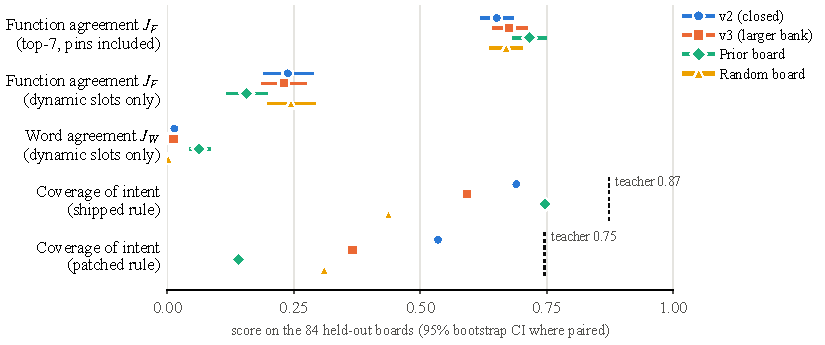
\includegraphics[width=\linewidth]{fig_axes.pdf}
\caption{Clean students and both baselines on the 84 test boards:
function agreement with and without the pinned slots, word agreement,
and coverage of intent under both rules (Table~\ref{tab:axes}; whiskers
are 95\,\% paired bootstrap intervals; coverage points have none).}
\label{fig:axes}
\end{figure}

\section{The second partition}
\label{app:val}

We apply the same metrics to the 84 validation rows. These are disjoint
from the test rows but guided early stopping for both students, which may
favour student performance on this partition. Coverage is scored on
$n=72$ rows; the 12 unscored rows have no authored acceptable moves.
Here the shipped distinct-functions gate is failed by v2 (0.806), the
prior (0.857) and the random board (0.844) and passed by v3 (1.010).
The last block pools the test and validation partitions ($n=168$);
because the validation rows guided early stopping this is exploratory.
Bootstrap intervals as in the main text.

\begin{table}[h]
\centering
\footnotesize
\caption{Aggregates on the 84 validation boards, same layout as
Table~\ref{tab:axes}.}
\label{tab:val}
\begin{tabular}{@{}lllll@{}}
\toprule
Metric & v2 (closed) & v3 (larger bank) & Prior & Random \\
\midrule
$J_F$ [95\,\% CI] & 0.670 [.64,.70] & 0.694 [.66,.73] & 0.706 [.67,.74] & 0.642 [.61,.67] \\
distinct-functions retention & 0.806 & 1.010 & 0.857 & 0.844 \\
same-fn.-pair (T 0.143) & 0.206 & 0.138 & 0.191 & 0.193 \\
$J_W$ [95\,\% CI] & 0.026 [.01,.04] & 0.010 [.00,.02] & 0.061 [.04,.08] & 0.007 [.00,.02] \\
dynamic-word overlap & 0.056 & 0.020 & 0.115 & 0.020 \\
board variety & 0.905 & 0.940 & 0.012 & 1.000 \\
coverage, shipped rule (teacher 0.861) & 0.639 & 0.597 & 0.736 & 0.486 \\
\quad margin verdict & fail & fail & inconcl. & fail \\
coverage, patched rule (teacher 0.681) & 0.486 & 0.361 & 0.167 & 0.347 \\
\quad margin verdict & inconcl. & fail & fail & fail \\
\midrule
\emph{I-don't-know} presence (T 0.512) & 0.143 $[-.50,-.24]$ & 1.000 $[+.38,+.60]$ & 1.000 & 0.226 \\
\emph{emotion} presence (T 0.381) & 0.012 $[-.48,-.26]$ & 0.167 $[-.32,-.11]$ & 0.000 & 0.048 \\
\midrule
\multicolumn{5}{@{}l}{\emph{Pooled over both partitions, $n=168$}} \\
$J_F$ [95\,\% CI] & 0.661 [.64,.68] & 0.685 [.66,.71] & 0.711 [.69,.74] & 0.656 [.63,.68] \\
$J_W$ [95\,\% CI] & 0.020 [.01,.03] & 0.011 [.01,.02] & 0.062 [.05,.08] & 0.005 [.00,.01] \\
\emph{I-don't-know} presence (T 0.464) & 0.173 $[-.39,-.20]$ & 1.000 $[+.46,+.61]$ & 1.000 & 0.226 \\
\emph{emotion} presence (T 0.381) & 0.018 $[-.44,-.29]$ & 0.161 $[-.30,-.14]$ & 0.000 & 0.048 \\
\bottomrule
\end{tabular}
\end{table}

\section{Configuration}
\label{app:config}

\textbf{Teacher.}
Qwen2.5-3B-Instruct, 4-bit, run locally through MLX with greedy decoding;
one fixed prompt per turn proposes candidate phrases; a symbolic MMR
stage (relevance--diversity trade-off $\lambda=0.6$, $\lambda=0.35$ for
the answer quota) selects six.
\textbf{Context encoder.}
\texttt{sentence-transformers/all-MiniLM-L6-v2}, L2-normalised, frozen;
used identically for the students' input, vocabulary deduplication, the
function labeller and the coverage matcher.
\textbf{Student v2.}
LayerNorm $\to$ Linear($769{\to}192$) $\to$ ReLU $\to$ Dropout(0.3)
$\to$ Linear($192{\to}45$), about 158k parameters; target is the multi-hot
set of the teacher's dynamic board words; loss is BCE with positive
weighting and frequency logit adjustment plus an auxiliary listwise term;
AdamW, lr $10^{-3}$, weight decay $10^{-3}$, batch 32, at most 60 epochs,
early stopping on validation loss with patience 15, seed 0.
Vocabulary: teacher dynamic words with frequency $\ge 3$ on the 391
training rows, deduplicated by single-link cosine $\ge 0.80$; class
weights and logit-adjustment priors from the training rows.
\textbf{Student v3.}
Two towers of the same LayerNorm--Linear--ReLU--Dropout--Linear shape
projecting context (769-d) and phrase (384-d MiniLM) into a shared 128-d
space; score is the dot product; BCE-with-logits over each batch's
in-batch positives plus 128 random bank negatives; same optimiser and
stopping rule. Bank: every teacher dynamic phrase on the training rows,
no frequency floor, deduplicated by complete-link cosine $\ge 0.85$.
The served builds differ only in using all 559 rows for the vocabulary,
the bank and the class statistics.
\textbf{Policy.}
Hedge cap 1 per board (0 when an open answer is present); answer reserve
2 slots when the partner asked a question; the hedge cluster is one
shared list of 17 phrases.
\textbf{Evaluator.}
Nine function exemplar sets, nearest exemplar by cosine, no abstention;
coverage lexical leg is a shared content token or word-boundary
substring, semantic leg cosine $\ge 0.50$; gates: distinct-functions
retention $\ge 0.90$, coverage $\ge 0.90\times$ teacher with a paired
bootstrap verdict, 10\,000 resamples, seed 0.

\section{Inventory leakage: the served build}
\label{app:prov}

The served students' inventories were built over all 559 rows before the
split. Rebuilding from the 391 training rows with the same floors and
deduplication gives the counts in the first table; the full-bank and
training-bank sets are not nested (complete-link deduplication changes
cluster representatives), so ``entries that need held-out rows'' exceeds
the size difference. Held-out means validation and test together;
Table~\ref{tab:served} sets the served build beside the clean one.

\begin{table}[h]
\centering
\small
\begin{tabular}{@{}lrr@{}}
\toprule
 & v2 label set & v3 phrase bank \\
\midrule
Built over all 559 rows (served) & 95 & 1\,959 \\
Built over the 391 training rows (clean) & 45 & 1\,447 \\
Served entries that need held-out rows to reach the floor & 50 & 546 \\
Test-window teacher items (of 252) in those entries & 28 & 150 \\
Test-window items representable from the clean build & --- & 100 \\
\bottomrule
\end{tabular}
\end{table}

\begin{table}[h]
\centering
\footnotesize
\caption{Served (all-rows inventory) versus clean (training-only inventory)
students on the 84 test boards. Random boards are drawn from the
respective v2 label space.}
\label{tab:served}
\begin{tabular}{@{}lrrrr@{}}
\toprule
Metric & v2 served & v2 clean & v3 served & v3 clean \\
\midrule
label set / bank size & 95 & 45 & 1\,959 & 1\,447 \\
$J_F$ (pins included) & 0.678 & 0.651 & 0.718 & 0.676 \\
$J_F^{\mathrm{dyn}}$ & 0.273 & 0.238 & 0.365 & 0.230 \\
$J_W$ & 0.032 & 0.014 & 0.067 & 0.012 \\
distinct-functions retention & 0.953 & 0.909 & 1.091 & 1.116 \\
coverage, patched rule & 0.620 & 0.535 & 0.620 & 0.366 \\
\emph{emotion} presence (teacher 0.381) & 0.167 & 0.024 & 0.345 & 0.155 \\
\emph{I-don't-know} presence (teacher 0.417) & 0.155 & 0.202 & 0.690 & 1.000 \\
\bottomrule
\end{tabular}
\end{table}

\section{Reproducing the analysis}
\label{app:repro}

One script builds each candidate board for every held-out row (students
via their production inference paths, baselines as defined in
\S\ref{sec:setting}), pairs it with the teacher's cached board, labels
both top-7 windows with the nearest-exemplar classifier, and accumulates
presence, slots, lexical overlap, the two Jaccard indices and the slot
confusion; a second mode runs the system's unchanged gate code (including
coverage of intent) over the same boards. A split flag selects the test
or the validation partition. Bootstrap intervals use 10\,000 resamples
and a fixed seed. An artefact-directory option selects the served or
clean build; the served v2 rows reproduce the committed gate values
(retention 0.953, dynamic-word overlap 0.067) exactly.
Representability counts (\S\ref{sec:causes}) are membership tests against
the label list and its deduplication map; scripts and tests will be
released with the camera-ready.

\end{document}
